\documentclass[11pt,letterpaper]{article}
\usepackage[margin=0.6in]{geometry}
\usepackage{amsmath,amssymb}
\usepackage{tikz}
\usetikzlibrary{arrows.meta,positioning}
\usepackage{xcolor}
\usepackage{fontawesome5}
\usepackage{tcolorbox}
\usepackage{multicol}
\usepackage{enumitem}
\usepackage{hyperref}

\definecolor{primaryblue}{RGB}{41, 98, 255}
\definecolor{accentgreen}{RGB}{0, 150, 136}
\definecolor{warnorange}{RGB}{255, 152, 0}
\definecolor{lightgray}{RGB}{245, 245, 245}
\definecolor{capstonecolor}{RGB}{156, 39, 176}

\tcbset{
    conceptbox/.style={colback=capstonecolor!5, colframe=capstonecolor, boxrule=1pt, arc=3pt, left=5pt, right=5pt, top=5pt, bottom=5pt},
    formulabox/.style={colback=lightgray, colframe=gray!50, boxrule=0.5pt, arc=2pt, left=5pt, right=5pt, top=3pt, bottom=3pt},
    stepbox/.style={colback=accentgreen!5, colframe=accentgreen, boxrule=1pt, arc=3pt, left=5pt, right=5pt, top=5pt, bottom=5pt},
    appbox/.style={colback=primaryblue!5, colframe=primaryblue, boxrule=1pt, arc=3pt, left=5pt, right=5pt, top=5pt, bottom=5pt}
}

\pagestyle{empty}
\setlength{\parindent}{0pt}
\setlist[itemize]{leftmargin=*, itemsep=1pt, topsep=2pt}
\setlist[enumerate]{leftmargin=*, itemsep=1pt, topsep=2pt}

\begin{document}

\begin{center}
{\LARGE\bfseries\color{capstonecolor} Capstone: Build PCA from Scratch}\\[3pt]
{\large Integrating Linear Algebra, Statistics, and Numerical Methods}
\end{center}
\vspace{-5pt}
\hrule height 2pt
\vspace{8pt}

\begin{multicols}{2}

\begin{tcolorbox}[conceptbox, title={\faTrophy\ Learning Goals}]
\begin{itemize}
    \item Implement PCA using \textbf{eigendecomposition}
    \item Implement PCA using \textbf{SVD}
    \item Understand why both approaches give same result
    \item Apply to real data (MNIST digits)
    \item Validate against sklearn
\end{itemize}
\end{tcolorbox}

\begin{tcolorbox}[stepbox, title={\faListOl\ Implementation Steps}]
\begin{enumerate}
    \item \textbf{Center the data}: $X_c = X - \bar{X}$
    \item \textbf{Compute covariance}: $C = \frac{1}{n-1} X_c^T X_c$
    \item \textbf{Eigendecomposition}: $C = V \Lambda V^T$
    \item \textbf{Sort by eigenvalue}: Largest first
    \item \textbf{Project}: $Z = X_c V_k$ (top $k$ eigenvectors)
    \item \textbf{Reconstruct}: $\hat{X} = Z V_k^T + \bar{X}$
\end{enumerate}
\end{tcolorbox}

\columnbreak

\begin{tcolorbox}[formulabox, title={\faCalculator\ Key Formulas}]
\textbf{Covariance Matrix:}
\[ C = \frac{1}{n-1} X_c^T X_c \]

\textbf{Explained Variance Ratio:}
\[ \text{ratio}_i = \frac{\lambda_i}{\sum_j \lambda_j} \]

\textbf{SVD Approach:}
\[ X_c = U \Sigma V^T \Rightarrow \text{PCs} = V \]

\textbf{Eigenvalues from SVD:}
\[ \lambda_i = \frac{\sigma_i^2}{n-1} \]
\end{tcolorbox}

\begin{tcolorbox}[appbox, title={\faLink\ Concepts Used}]
\begin{itemize}
    \item \textbf{Ch 1}: Matrix multiplication, eigenvalues
    \item \textbf{Ch 2}: Variance, covariance
    \item \textbf{Ch 6}: SVD, low-rank approximation
    \item \textbf{Ch 7}: Projections, basis change
    \item \textbf{Ch 8}: Numerical stability
\end{itemize}
\end{tcolorbox}

\end{multicols}

\vspace{3pt}

\begin{center}
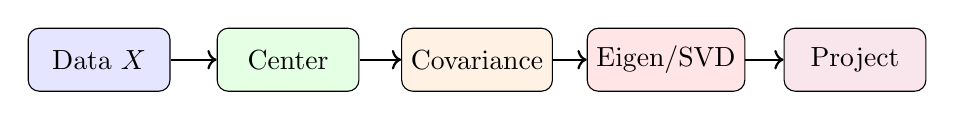
\begin{tikzpicture}[scale=0.8]
    % Pipeline visualization
    \node[draw, rounded corners, fill=blue!10, minimum width=1.8cm, minimum height=0.8cm] (data) at (0,0) {Data $X$};
    \node[draw, rounded corners, fill=green!10, minimum width=1.8cm, minimum height=0.8cm] (center) at (3,0) {Center};
    \node[draw, rounded corners, fill=orange!10, minimum width=1.8cm, minimum height=0.8cm] (cov) at (6,0) {Covariance};
    \node[draw, rounded corners, fill=red!10, minimum width=1.8cm, minimum height=0.8cm] (eig) at (9,0) {Eigen/SVD};
    \node[draw, rounded corners, fill=purple!10, minimum width=1.8cm, minimum height=0.8cm] (proj) at (12,0) {Project};

    \draw[->,thick] (data) -- (center);
    \draw[->,thick] (center) -- (cov);
    \draw[->,thick] (cov) -- (eig);
    \draw[->,thick] (eig) -- (proj);
\end{tikzpicture}
\end{center}

\vspace{5pt}
\hrule
\vspace{5pt}

\begin{center}
\faGithub\ \textbf{Notebook}: \url{https://github.com/vijaygwu/math-powers-ai/blob/main/notebooks/capstone_pca.ipynb}
\end{center}

\end{document}
